
The flow around a flat airfoil is one of the few cases for which analytical solutions are possible.
Following the work by Theodore Theodorsen, we analyze the flow past a flat plate with both heaving and pitching motion, and further find the optimal stroke for maximum energy extraction from the ambient flow. 

\section{Flow past a flat plate}

The flow can be decomposed into two parts: noncirculatory flow, and circulatory flow due to vortex shedding.
With those, the forces and moments acting on the airfoil, and then the total work done by the fluid on the plate, are calculated.

\subsection{Noncirculatory flow}

In this part, the velocity (potential) which satisfies the Laplace equaiton with the no-penetration boundary condition is calculated.
The flat plate with length $2b$ in $z-plane$ can be obtained from a circle with radius $b$ in $\zeta$-plane, through the Zhukovsky conformal mapping
\begin{align}
2z = \zeta + \frac{b^2}{\zeta},    \text{   or~~~~~~}   \zeta =z \pm \sqrt{z^2-b^2}.
\end{align}
Note that we have an extra fractor $2$ in front of $z$ and by this the plate is simply the projection of the circle on the  $x$ axis.
But when we transform the flow back into that $z$-plane, the free stream velocity at infinity should be reduced by half.
As we know, the complex flow potential around a 2D circular cylinder with radius $b$ placed in an otherwise free stream $(u,v)$ is the superposition of potentials of the free stream and the flow due to a dipole 
\begin{align}
w(\zeta) = (u-iv)\zeta+\frac{(u+iv)b^2}{\zeta}.
\end{align} 
Plugging the Zhukovsky mapping in (remember to reduce the free stream velocity by half), we get the flow around the flat plate as
\begin{align}
w(z) = uz \mp iv\sqrt{z^2-b^2}.
\end{align} 
For the calculation of the forces and moments on the plate, we only need the flow on the surface of the plate.
Let $z = bx$ with $x$ dimensionless, and we get the potential as
\begin{align}
\phi(x) = ubx \pm vb\sqrt{1-x^2},
\end{align} 
where the plus and minus signs correspond to the upper and lower surfaces respectively. 
The first term is due to the free stream, and is common for both surfaces, thus contributing nothing to the total forces and moments on the airfoil as a whole.
In the following, potential $\phi$ will only refer to the perturbation to the free stream on the upper surface of the airfoil
\begin{align}
\phi(x) = vb\sqrt{1-x^2}.
\end{align} 
Apply this to the flat airfoil, lying with a small angle $\alpha$ relative to the horizontal level, moving horizontally with speed $v$ and also vertically with speed $\dot{h}$. Relative to the airfoil, the free stream is $(v,v\alpha+\dot{h})$ and the corresponding potential is
\begin{align}
\phi(x) = (v\alpha + \dot{h})b\sqrt{1-x^2}.
\end{align} 
However, if $\alpha$ is not a constant, we have another contribution from rotation $\dot{\alpha}bx$ of the plate, which can be obtained by the summation of flow due to the motion of each infinitesimal element of the plate (???).
This contribution turns out to be $\phi(x) = \frac{1}{2}\dot{\alpha}xb^2\sqrt{1-x^2}$, and so the total potential of noncirculatory part is
\begin{align}
\phi_{nc}(x) = (v\alpha + \dot{h} + \frac{1}{2}\dot{\alpha}bx) b\sqrt{1-x^2}.
\end{align} 

With he velocity potentials being known, we are able to calculate the local pressures and by integration to obtain the total forces and moments on the airfoil.
Employing the Bernoulli's equation for unsteady flow, the local pressure is, except for a constant,
\begin{align}
p_h = -\rho[\frac{\partial \phi}{\partial t} + \frac{q^2}{2}],
\end{align} 
where the local velocity is $q = v+\frac{\partial \phi}{\partial (bx)}$. Then we obtain the pressure difference between upper and lower surfaces at $x$ as
\begin{align}
p(x) = -2\rho(\frac{\partial \phi}{\partial t} + v\frac{\partial \phi}{\partial (bx)}).
\end{align} 
Finally, we are able to write down the total forces and moments acting on the airfoil due to noncirculatory part of the flow as
\begin{align}
P_{nc} & = \int^{1}_{-1}pbdx
   = -\pi\rho b^2(v\dot{\alpha} + \ddot{h})   \\
M_{nc} & = \int^{1}_{-1}pb^2xdx
   = -\pi\rho b^2[\frac{1}{8}b^2\ddot{\alpha}-v(v\alpha + \dot{h})].
\end{align}


\subsection{Circulatory flow}

In this part, we shall calculate the flow due to the shed vortices extending from the airfoil to infinity to account for the viscous effect.
As we know, the velocity potential of the flow around the circle (with radius 1) resulting from the vortex element $d\Gamma$ at $(X_0, 0)$ ($X_0 > 1$) can be obtained by the superposition of the flow due to the vortex and an image vortex $-d\Gamma$ at $(1/X_0,0)$ as
\begin{align}
\mathrm{d}\phi_\Gamma (X,Y) & = \frac{\mathrm{d}\Gamma}{2\pi}[\arctan \frac{Y}{X-X_0} - \arctan \frac{Y}{X-1/X_0}]  \\
            & =  \frac{\mathrm{d}\Gamma}{2\pi}\arctan \frac{(X_0-1/X_0)Y}{X^2-(X_0+1/X_0)X+Y^2+1}
\end{align}
Introducing $X_0 + 1/X_0 = 2x_0$ or $X_0 = x_0 + \sqrt{x_0^2-1}$ on the $x$ axis, and $X=x$ and $Y=\sqrt{1-x^2}$ on the circle (upper half), the potential becomes
\begin{align}
\mathrm{d}\phi (x) = \frac{\mathrm{d}\Gamma}{2\pi} \arctan \frac{\sqrt{1-x^2}\sqrt{x_0^2-1}}{1-x_0x}.
\end{align}
Since our Zhukovsky transformation exactly maps point $(X_0, 0)$ to $(x_0, 0)$ and points on a circle to its projection on the $x$-axis, the expression above gives precisely the potential at $x$ on a flat plate due to vortex element $d\Gamma$ at $(x_0, 0)$.

For the pressure difference between upper and lower surfaces, we have the same relation $p = -2\rho[\frac{\partial \phi}{\partial t} + v\frac{\partial \phi}{\partial (bx)}]$.
But since the vortex elements are regarded as moving to the right relative to the airfoil with the free stream velocity $v$,  we have $\frac{\partial \phi}{\partial t} = v\frac{\partial \phi}{\partial (bx_0)}$ and so 
\begin{align}
p & = -2\rho v[\frac{\partial \phi}{\partial (bx_0)} + \frac{\partial \phi}{\partial (bx)}]  \\
  &  = -\frac{\rho v \mathrm{d}\Gamma}{\pi b} \frac{x_0+x}{\sqrt{1-x^2}\sqrt{x_0^2-1}}.
\end{align}
By integration over all the vortices and with $d\Gamma = U(x_0)bdx_0$, we get the distribution of potential and pressure difference on the plate with respect to the line vortex density $U(x_0)$ as follows,
\begin{align}
\phi_c(x) & =  \frac{1}{2\pi} \int_{1}^{\infty}\arctan \frac{\sqrt{1-x^2}\sqrt{x_0^2-1}}{1-x_0x}U\mathrm{d}x_0, \\
p_c(x) &  =  -\frac{\rho v }{\pi b} \int_{1}^{\infty}\frac{x_0+x}{\sqrt{1-x^2}\sqrt{x_0^2-1}} Ub\mathrm{d}x_0.
\end{align}
With further integration over the plate, the total force and moment acting on the airfoil are obtained as
\begin{align}
P_c & =  \int_{-1}^{1} p(x) b \mathrm{d}x
   =  -\rho v b \int_{1}^{\infty} \frac{x_0}{\sqrt{x_0^2-1}} U \mathrm{d}x_0, \\
M_c & =  \int_{-1}^{1} p(x) b^2 x \mathrm{d}x
   =   - \frac{1}{2} \rho v b^2 \int_{1}^{\infty} \frac{1}{\sqrt{x_0^2-1}} U \mathrm{d}x_0.
\end{align}
Note that since the vortex element is considered stationary with respect to the fluid elements, we have $U(x_0) = f(vt - x_0)$, where $t$ is the time since the beginning of the motion and $vt-x_0$ is the distance from the location of the first vortex element.


\subsection{Magnitude of Circulation}

In this section, the magnitude of the circulation is determined by the Kutta condition, which requires that no infinite velocities exist at the trailing edge of the plate, or at $x = 1$,
\begin{align}
\frac{\partial (\phi_{nc} + \phi_c)}{\partial x} |_{x = 1} = \text{finite}.
\end{align}
Introducing the expression for $\phi_{nc}$ and $\phi_c$ from the previous two parts gives the following relation
\begin{align}       \label{eqn:Kutta}
\frac{1}{2\pi} \int_{1}^{\infty} \sqrt{\frac{x_0+1}{x_0-1}} U \mathrm{d}x_0 = v\alpha + \dot{h} + \frac{1}{2}b\dot{\alpha}.
\end{align}
For our purpose, the variables on the right hand side, say $\alpha$ and $\dot{h}$, are given and the circulation $U(x_0)$ is determined by the relation above, and the flow around the airfoil is further obtained. 
In the following, we write
\begin{align}
Q \equiv v\alpha + \dot{h} + \frac{1}{2}b\dot{\alpha},
\end{align}
and introduce the function
\begin{align}
C(k) \equiv \frac{\int_{1}^{\infty} \frac{x_0}{\sqrt{x_0^2-1}} U \mathrm{d}x_0}{\int_{1}^{\infty} \frac{x_0+1}{\sqrt{x_0^2-1}} U \mathrm{d}x_0}.
\end{align}
By these, the force and moment acting on the airfoil due to the circulatory flow can be rewritten as
\begin{align}
P_c & = -2\pi \rho b v CQ,  \\
M_c & = \pi \rho b^2 v (C-1)Q.
\end{align}

\subsection{Function C(k)}

If the airfoil adjusts its configuration periodically, that is, the variables $\alpha$ and $h$ are both periodic functions of time with a single mode, we can write the circulation as $U = U_0 \exp \{i[k(\frac{s}{b}-x_0)+ \varphi] \}$, where $s = vt$ denotes the distance from the first vortex element to the airfoil, and $k$ is the dimensionless wavenumber.
For this special case with a single mode, we don't need to calculate the magnitude $U_0$ explicitly using the relation (\ref{eqn:Kutta}), because it will cancel out in $C(k)$ and give
\begin{align}
C(k) = \frac{\int_{1}^{\infty} \frac{x_0}{\sqrt{x_0^2-1}} e^{-ikx_0} \mathrm{d}x_0}{\int_{1}^{\infty} \frac{x_0+1}{\sqrt{x_0^2-1}} e^{-ikx_0} \mathrm{d}x_0}.
\end{align}
The integrals on the numerator and denominator can both be expressed using Bessel functions, and then the equation can be written as
\begin{align}
C(k) & =  \frac{\frac{\pi}{2}(-J_1+iY_1)}{\frac{\pi}{2}(-(J_1+Y_0)+i(Y_1-J_0))}
          \equiv  F+iG,
\end{align}
with the real and imaginary part
\begin{align}
F & = \frac{J_1(J_1+Y_0)+Y_1(Y_1-J_0)}{(J_1+Y_0)^2+(Y_1-J_0)^2},  \\
G & = -\frac{Y_1Y_0+J_1J_0}{(J_1+Y_0)^2+(Y_1-J_0)^2}.
\end{align}
For general motion of the airfoil, we can write $Q$  and $U$ as the superposition of different modes and then relate the magnitude of each mode through relation (\ref{eqn:Kutta}). In that case, the magnitude of each mode of the circulation will explicitly appear in the expression of $C(k)$.


\section{Optimal Efficiency for Energy Extraction}

In this part, we will optimize the airfoil strokes for maximum energy extracted from the ambient flow, subject to the constraint that the energy cost for adjusting the configuration of the airfoil is given.

For simplicity, we assume the airfoil moves with a periodic pitching and heaving, that is,
\begin{align}
\alpha = Re(A e^{i\omega t}),    \text{    and   }        h = Re(bH e^{i\omega t}),
\end{align}
with the complex amplitudes $A$ and $H$ dimensionless.

First, we can easily see that the work done by the noncirculatory flow on the airfoil averaged over one period is zero. The work rate is
\begin{align}
W_{nc} & =  P_{nc} \dot{h} + M_{nc} \dot{\alpha}  \\
       & =  \pi \rho b^2 (v^2 \alpha \dot{\alpha} - \frac{1}{8} b^2 \dot{\alpha} \ddot{\alpha} - \dot{h} \ddot{h})  \\
       & =  \pi \rho b^2 \frac{1}{2} \frac{d}{dt} (v^2 {\alpha}^2 - \frac{1}{8} b^2 {\dot{\alpha}}^2 - {\dot{h}}^2 ),
\end{align}
and the corresponding average value vanishes obviously, that is
\begin{align}
\overline{W}_{nc} = \frac{\omega}{2\pi} \int_{0}^{2\pi/\omega} W_{nc} \mathrm{d}t = 0.
\end{align}
Then the work done by the circulatory flow is
\begin{align}
W_{c}  = & P_{c} \dot{h} + M_{c} \dot{\alpha}  \\
        = & -2\pi \rho b v Re(CQ) Re(i\omega bH e^{i\omega t}) + \pi \rho b^2 v Re((C-1)Q) Re(i\omega A e^{i\omega t})  \\
    = & -2\pi \rho b v \frac{1}{4} [ C(vA+i\omega bH + \frac{1}{2} i\omega bA)i\omega bH e^{i2\omega t} + c.c. \\
       &  + C(vA+i\omega bH + \frac{1}{2} i\omega bA) (-i\omega bH^{*}) + c.c.]  \\
      &  +\pi \rho b^2 v \frac{1}{4} [ (C-1)(vA+i\omega bH + \frac{1}{2} i\omega bA)i\omega A e^{i2\omega t} + c.c. \\
      &   + (C-1)(vA+i\omega bH + \frac{1}{2} i\omega bA) (-i\omega A^{*}) + c.c.],
\end{align}
and averaging over one period, noticing that the first and third line contribute nothing, gives 
\begin{align}
\overline{W}_{c}  = & -2\pi \rho b v \frac{1}{4} [C(vA+i\omega bH + \frac{1}{2} i\omega bA) (-i\omega bH^{*}) + c.c.]     \\
                                  & +\pi \rho b^2 v \frac{1}{4} [(C-1)(vA+i\omega bH + \frac{1}{2} i\omega bA) (-i\omega A^{*}) + c.c.]
\end{align}
Considering  $\omega = \frac{vk}{b}$, the expression above can be rewritten with standard quadratic form as
\begin{align}
\frac{\overline{W}_{c}}{ \pi \rho v^3 b/4} = \overline{X} M X,
\end{align}
with
\begin{align}
X =  \begin{bmatrix} H  \\  A   \end{bmatrix},
M = \begin{bmatrix}   -4k^2 F   &  -k(2G+k) - i2k(kG-F)  \\
                         -k(2G+k) + i2k(kG-F)  &   k^2(F-1)+2kG  \end{bmatrix}.
\end{align}
Remember that the energy cost for the airfoil is given, say, $\overline{X} X = 1$.
So our goal is to maximize $\overline{X} M X$ under the constraint $\overline{X} X = 1$.
It is readily shown that this is equivalent to solve the eigenvalue problem of $M$ as follows.
The objective function with Lagrangian multiplier is 
\begin{align}
f(X; \lambda) = \overline{X} M X - \lambda (\overline{X} X - 1),
\end{align}
and setting the derivative as zero gives $MX = \lambda X$ and the corresponding extreme value of $f$ is found to be $\lambda$.

\subsection{Asymptotic analysis}

For small $x$, the Bessel's functions have the following asymtotes
\begin{align}
Y_0(x)  \simeq  \frac{2}{\pi}[\ln (\frac{x}{2}) + \gamma],   \hspace{20pt}  J_0(x) \simeq 1  \\
Y_1(x)  \simeq  -\frac{2}{\pi x},   \hspace{40pt}  J_1(x) \simeq \frac{x}{2}
\end{align}
where $\gamma \simeq 0.5772$ is the Euler-Mascheroni constant, and accordingly
\begin{align}
F(k) \simeq 1,  \hspace{30pt}   G(k) \simeq k \ln (\frac{k}{2})
\end{align}
and
\begin{align}
M \simeq \begin{bmatrix}   -4k^2   &  -k^2[1+ 2\ln (\frac{k}{2})] + i2k[1-k^2\ln (\frac{k}{2})]  \\
                        -k^2[1+ 2\ln (\frac{k}{2})] - i2k[1-k^2\ln (\frac{k}{2})] &   2k^2\ln (\frac{k}{2})  \end{bmatrix}.
\end{align}
With these approximations, the maximum eigenvalue and the corresponding eigenvector are found to be
\begin{align}
\lambda_{max} \simeq 2k,   \hspace{1cm}
X \simeq   \frac{1}{\sqrt{2}}
\begin{bmatrix} -k \ln k + i \\  1   \end{bmatrix}.
\end{align}
We see that in this low-frequency regime the optimal stroke has a phase difference between pitching and hitching, which tends to $\pi/2$ as $k$ goes to 0, and the corresponding optimal energy coefficient is linearly proportional to the frequency.

For large $x$, the Bessel's functions have different approximations from the case of small $x$ as
\begin{align}
Y_0(x) & \simeq  \sqrt{\frac{2}{\pi x}} [ \sin (x-\frac{\pi}{4}) - \frac{1}{8x} \cos (x - \frac{\pi}{4}) ], \\
Y_1(x) & \simeq  \sqrt{\frac{2}{\pi x}} \large{[} -\cos (x-\frac{\pi}{4})+\frac{3}{8x} \cos (x - \frac{\pi}{4}) \large{]}, \\
J_0(x) & \simeq  \sqrt{\frac{2}{\pi x}} \large{[} \cos (x-\frac{\pi}{4}) + \frac{1}{8x} \sin (x - \frac{\pi}{4}) \large{]}, \\
J_1(x) & \simeq  \sqrt{\frac{2}{\pi x}} \large{[} \sin (x-\frac{\pi}{4}) + \frac{3}{8x} \cos (x - \frac{\pi}{4}) \large{]},
\end{align}
and accordingly
\begin{align}
F(k) \simeq \frac{1}{2},   \hspace{25pt}  G(k) \simeq -\frac{1}{8k}
\end{align}
and
\begin{align}
M \simeq \begin{bmatrix}   -2k^2   &  (-k^2+\frac{1}{4}) + i\frac{5}{4}k  \\
                        (-k^2+\frac{1}{4}) - i\frac{5}{4}k &   -\frac{1}{2}k^2-\frac{1}{4}  \end{bmatrix}.
\end{align}
In this case, the maximum eigenvalue and the corresponding eigenvector are found to be
\begin{align}
\lambda_{max} = \frac{9}{40} + O(\frac{1}{k^2}), \hspace{1cm}
X \simeq \frac{2}{\sqrt{5}}
\begin{bmatrix} \frac{1}{2} - i \frac{5}{8k}   \\     -1     \end{bmatrix}.
\end{align}
We see that in this high-frequency regime the maximum efficiency of energy extraction tends to a constant as the frequency grows.

\subsection{Numerical solution}

\begin{figure}
\begin{center}
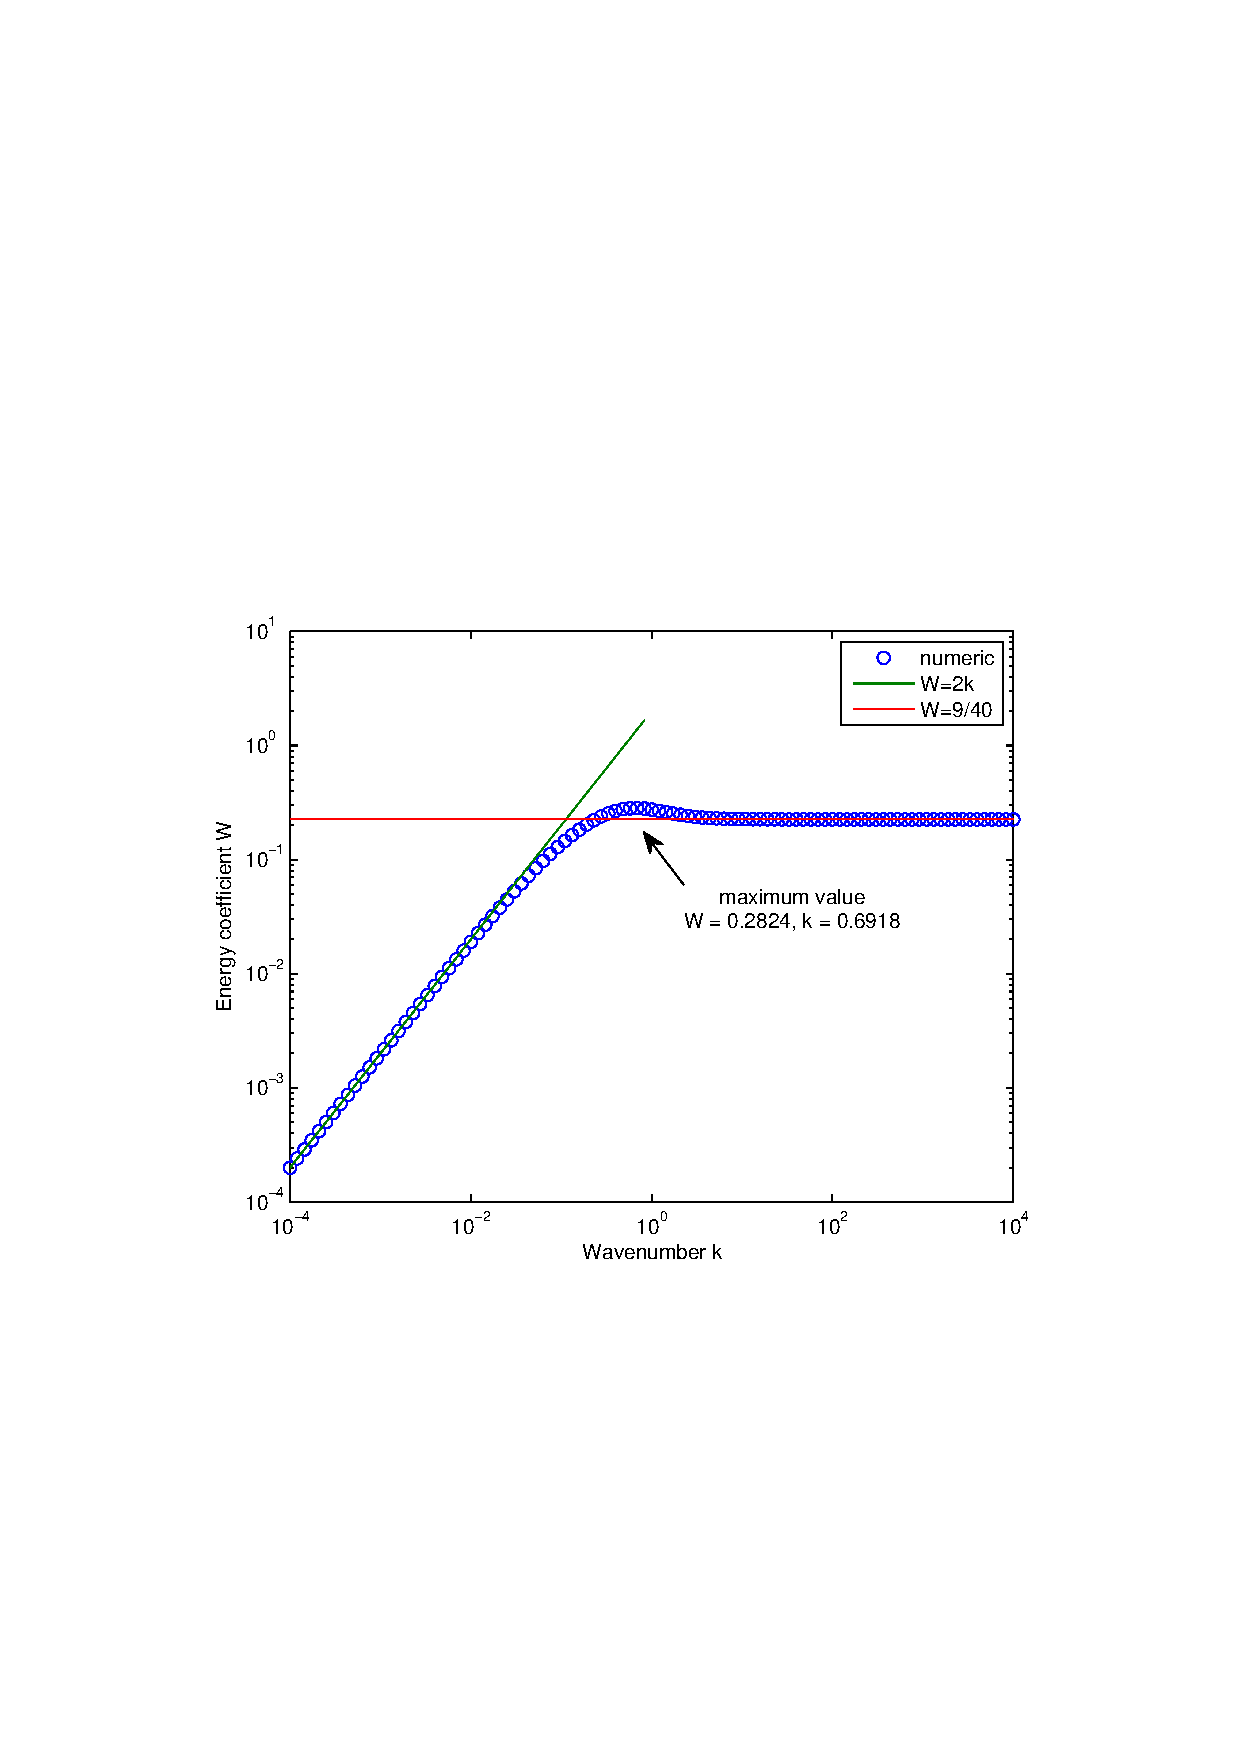
\includegraphics[width=12cm]{Figures/TheodorsenEnergy.pdf}
\caption[The optimal energy efficient for different stroke frequencies]{The optimal efficiency of energy extraction for different stroke frequencies is shown. The two different asymptotic behaviors are captured.}
\end{center}
\end{figure}
